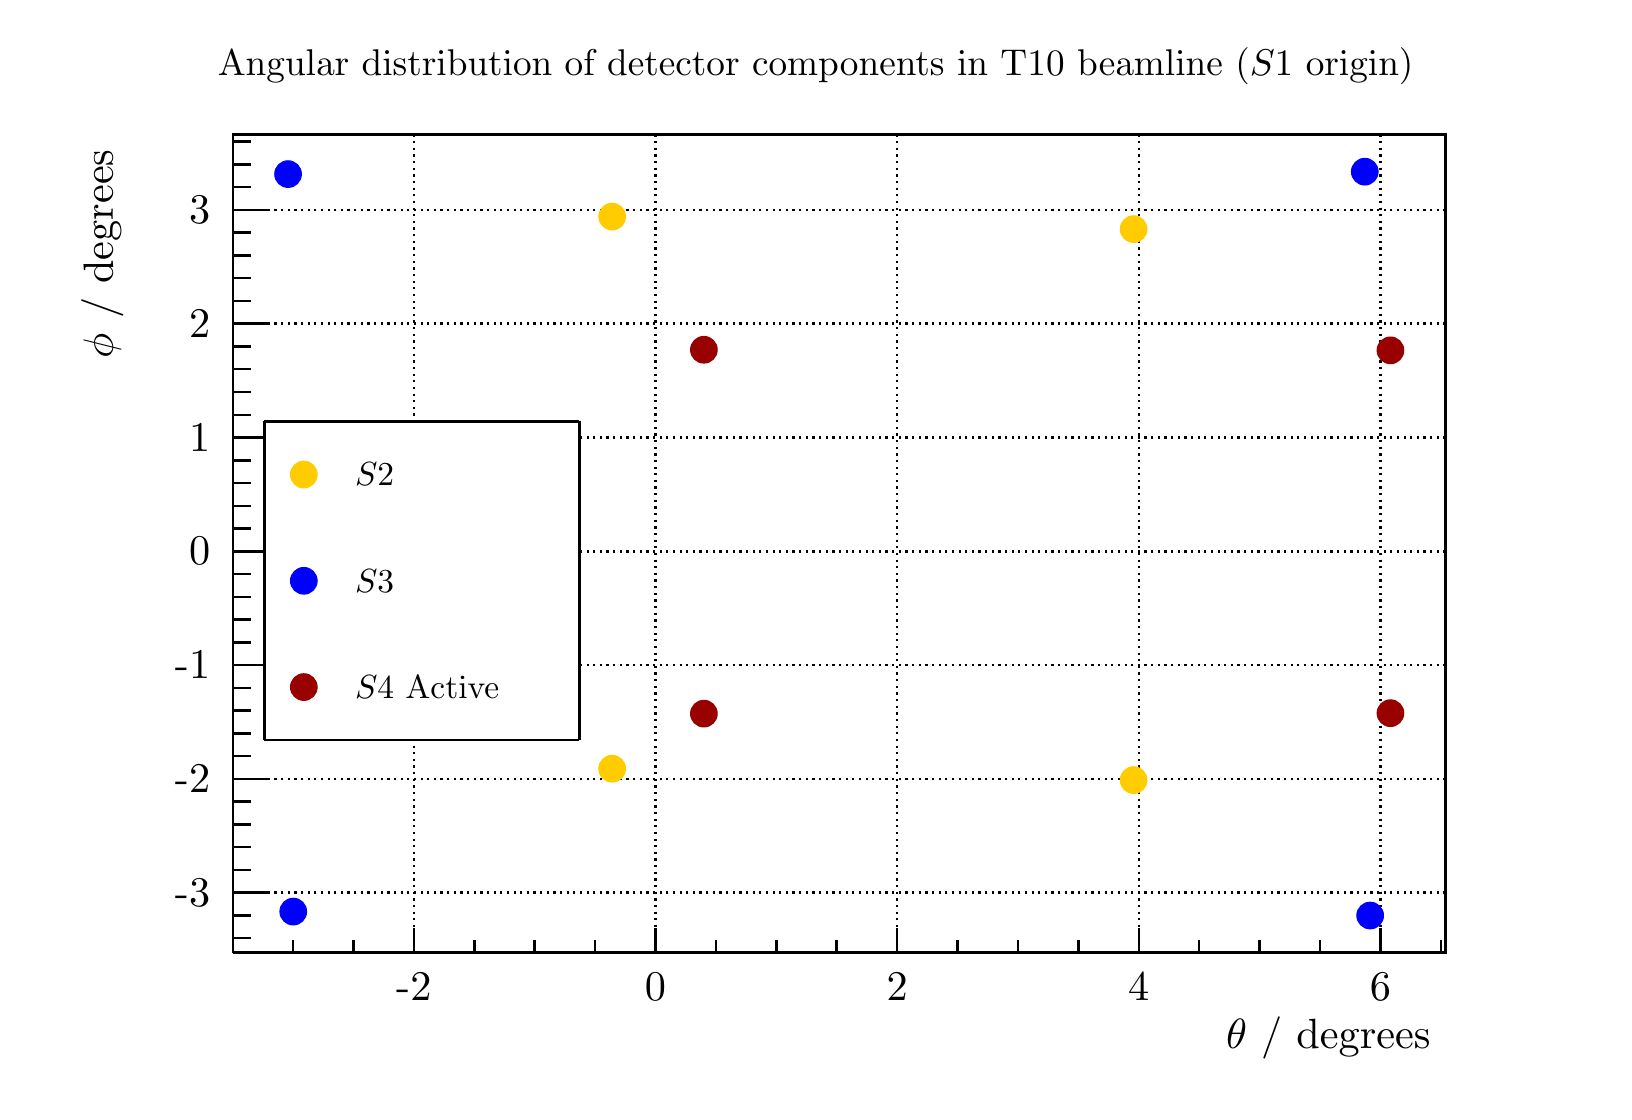
\begin{tikzpicture}
\pgfdeclareplotmark{cross} {
\pgfpathmoveto{\pgfpoint{-0.3\pgfplotmarksize}{\pgfplotmarksize}}
\pgfpathlineto{\pgfpoint{+0.3\pgfplotmarksize}{\pgfplotmarksize}}
\pgfpathlineto{\pgfpoint{+0.3\pgfplotmarksize}{0.3\pgfplotmarksize}}
\pgfpathlineto{\pgfpoint{+1\pgfplotmarksize}{0.3\pgfplotmarksize}}
\pgfpathlineto{\pgfpoint{+1\pgfplotmarksize}{-0.3\pgfplotmarksize}}
\pgfpathlineto{\pgfpoint{+0.3\pgfplotmarksize}{-0.3\pgfplotmarksize}}
\pgfpathlineto{\pgfpoint{+0.3\pgfplotmarksize}{-1.\pgfplotmarksize}}
\pgfpathlineto{\pgfpoint{-0.3\pgfplotmarksize}{-1.\pgfplotmarksize}}
\pgfpathlineto{\pgfpoint{-0.3\pgfplotmarksize}{-0.3\pgfplotmarksize}}
\pgfpathlineto{\pgfpoint{-1.\pgfplotmarksize}{-0.3\pgfplotmarksize}}
\pgfpathlineto{\pgfpoint{-1.\pgfplotmarksize}{0.3\pgfplotmarksize}}
\pgfpathlineto{\pgfpoint{-0.3\pgfplotmarksize}{0.3\pgfplotmarksize}}
\pgfpathclose
\pgfusepathqstroke
}
\pgfdeclareplotmark{cross*} {
\pgfpathmoveto{\pgfpoint{-0.3\pgfplotmarksize}{\pgfplotmarksize}}
\pgfpathlineto{\pgfpoint{+0.3\pgfplotmarksize}{\pgfplotmarksize}}
\pgfpathlineto{\pgfpoint{+0.3\pgfplotmarksize}{0.3\pgfplotmarksize}}
\pgfpathlineto{\pgfpoint{+1\pgfplotmarksize}{0.3\pgfplotmarksize}}
\pgfpathlineto{\pgfpoint{+1\pgfplotmarksize}{-0.3\pgfplotmarksize}}
\pgfpathlineto{\pgfpoint{+0.3\pgfplotmarksize}{-0.3\pgfplotmarksize}}
\pgfpathlineto{\pgfpoint{+0.3\pgfplotmarksize}{-1.\pgfplotmarksize}}
\pgfpathlineto{\pgfpoint{-0.3\pgfplotmarksize}{-1.\pgfplotmarksize}}
\pgfpathlineto{\pgfpoint{-0.3\pgfplotmarksize}{-0.3\pgfplotmarksize}}
\pgfpathlineto{\pgfpoint{-1.\pgfplotmarksize}{-0.3\pgfplotmarksize}}
\pgfpathlineto{\pgfpoint{-1.\pgfplotmarksize}{0.3\pgfplotmarksize}}
\pgfpathlineto{\pgfpoint{-0.3\pgfplotmarksize}{0.3\pgfplotmarksize}}
\pgfpathclose
\pgfusepathqfillstroke
}
\pgfdeclareplotmark{newstar} {
\pgfpathmoveto{\pgfqpoint{0pt}{\pgfplotmarksize}}
\pgfpathlineto{\pgfqpointpolar{44}{0.5\pgfplotmarksize}}
\pgfpathlineto{\pgfqpointpolar{18}{\pgfplotmarksize}}
\pgfpathlineto{\pgfqpointpolar{-20}{0.5\pgfplotmarksize}}
\pgfpathlineto{\pgfqpointpolar{-54}{\pgfplotmarksize}}
\pgfpathlineto{\pgfqpointpolar{-90}{0.5\pgfplotmarksize}}
\pgfpathlineto{\pgfqpointpolar{234}{\pgfplotmarksize}}
\pgfpathlineto{\pgfqpointpolar{198}{0.5\pgfplotmarksize}}
\pgfpathlineto{\pgfqpointpolar{162}{\pgfplotmarksize}}
\pgfpathlineto{\pgfqpointpolar{134}{0.5\pgfplotmarksize}}
\pgfpathclose
\pgfusepathqstroke
}
\pgfdeclareplotmark{newstar*} {
\pgfpathmoveto{\pgfqpoint{0pt}{\pgfplotmarksize}}
\pgfpathlineto{\pgfqpointpolar{44}{0.5\pgfplotmarksize}}
\pgfpathlineto{\pgfqpointpolar{18}{\pgfplotmarksize}}
\pgfpathlineto{\pgfqpointpolar{-20}{0.5\pgfplotmarksize}}
\pgfpathlineto{\pgfqpointpolar{-54}{\pgfplotmarksize}}
\pgfpathlineto{\pgfqpointpolar{-90}{0.5\pgfplotmarksize}}
\pgfpathlineto{\pgfqpointpolar{234}{\pgfplotmarksize}}
\pgfpathlineto{\pgfqpointpolar{198}{0.5\pgfplotmarksize}}
\pgfpathlineto{\pgfqpointpolar{162}{\pgfplotmarksize}}
\pgfpathlineto{\pgfqpointpolar{134}{0.5\pgfplotmarksize}}
\pgfpathclose
\pgfusepathqfillstroke
}
\definecolor{c}{rgb}{1,1,1};
\draw [color=c, fill=c] (0,0) rectangle (20,13.4957);
\draw [color=c, fill=c] (2.6,1.75444) rectangle (18,12.1461);
\definecolor{c}{rgb}{0,0,0};
\draw [c,line width=0.9] (2.6,1.75444) -- (2.6,12.1461) -- (18,12.1461) -- (18,1.75444) -- (2.6,1.75444);
\definecolor{c}{rgb}{1,1,1};
\draw [color=c, fill=c] (2.6,1.75444) rectangle (18,12.1461);
\definecolor{c}{rgb}{0,0,0};
\draw [c,line width=0.9] (2.6,1.75444) -- (2.6,12.1461) -- (18,12.1461) -- (18,1.75444) -- (2.6,1.75444);
\draw [c,line width=0.9] (2.6,1.75444) -- (18,1.75444);
\draw [c,dash pattern=on 0.80pt off 1.60pt ,line width=0.9] (4.89745,12.1461) -- (4.89745,1.75444);
\draw [c,dash pattern=on 0.80pt off 1.60pt ,line width=0.9] (7.96612,12.1461) -- (7.96612,1.75444);
\draw [c,dash pattern=on 0.80pt off 1.60pt ,line width=0.9] (11.0348,12.1461) -- (11.0348,1.75444);
\draw [c,dash pattern=on 0.80pt off 1.60pt ,line width=0.9] (14.1035,12.1461) -- (14.1035,1.75444);
\draw [c,dash pattern=on 0.80pt off 1.60pt ,line width=0.9] (17.1721,12.1461) -- (17.1721,1.75444);
\draw [c,dash pattern=on 0.80pt off 1.60pt ,line width=0.9] (4.89745,12.1461) -- (4.89745,1.75444);
\draw [c,dash pattern=on 0.80pt off 1.60pt ,line width=0.9] (17.1721,12.1461) -- (17.1721,1.75444);
\draw [c,line width=0.9] (2.6,1.75444) -- (2.6,12.1461);
\draw [c,dash pattern=on 0.80pt off 1.60pt ,line width=0.9] (18,2.51696) -- (2.6,2.51696);
\draw [c,dash pattern=on 0.80pt off 1.60pt ,line width=0.9] (18,3.96211) -- (2.6,3.96211);
\draw [c,dash pattern=on 0.80pt off 1.60pt ,line width=0.9] (18,5.40726) -- (2.6,5.40726);
\draw [c,dash pattern=on 0.80pt off 1.60pt ,line width=0.9] (18,6.85241) -- (2.6,6.85241);
\draw [c,dash pattern=on 0.80pt off 1.60pt ,line width=0.9] (18,8.29756) -- (2.6,8.29756);
\draw [c,dash pattern=on 0.80pt off 1.60pt ,line width=0.9] (18,9.74271) -- (2.6,9.74271);
\draw [c,dash pattern=on 0.80pt off 1.60pt ,line width=0.9] (18,11.1879) -- (2.6,11.1879);
\draw [c,dash pattern=on 0.80pt off 1.60pt ,line width=0.9] (18,2.51696) -- (2.6,2.51696);
\draw [c,dash pattern=on 0.80pt off 1.60pt ,line width=0.9] (18,11.1879) -- (2.6,11.1879);
\draw [c,line width=0.9] (2.6,1.75444) -- (18,1.75444);
\draw [c,line width=0.9] (4.89745,2.06619) -- (4.89745,1.75444);
\draw [c,line width=0.9] (5.66462,1.91032) -- (5.66462,1.75444);
\draw [c,line width=0.9] (6.43179,1.91032) -- (6.43179,1.75444);
\draw [c,line width=0.9] (7.19896,1.91032) -- (7.19896,1.75444);
\draw [c,line width=0.9] (7.96612,2.06619) -- (7.96612,1.75444);
\draw [c,line width=0.9] (8.73329,1.91032) -- (8.73329,1.75444);
\draw [c,line width=0.9] (9.50046,1.91032) -- (9.50046,1.75444);
\draw [c,line width=0.9] (10.2676,1.91032) -- (10.2676,1.75444);
\draw [c,line width=0.9] (11.0348,2.06619) -- (11.0348,1.75444);
\draw [c,line width=0.9] (11.802,1.91032) -- (11.802,1.75444);
\draw [c,line width=0.9] (12.5691,1.91032) -- (12.5691,1.75444);
\draw [c,line width=0.9] (13.3363,1.91032) -- (13.3363,1.75444);
\draw [c,line width=0.9] (14.1035,2.06619) -- (14.1035,1.75444);
\draw [c,line width=0.9] (14.8706,1.91032) -- (14.8706,1.75444);
\draw [c,line width=0.9] (15.6378,1.91032) -- (15.6378,1.75444);
\draw [c,line width=0.9] (16.405,1.91032) -- (16.405,1.75444);
\draw [c,line width=0.9] (17.1721,2.06619) -- (17.1721,1.75444);
\draw [c,line width=0.9] (4.89745,2.06619) -- (4.89745,1.75444);
\draw [c,line width=0.9] (4.13029,1.91032) -- (4.13029,1.75444);
\draw [c,line width=0.9] (3.36312,1.91032) -- (3.36312,1.75444);
\draw [c,line width=0.9] (17.1721,2.06619) -- (17.1721,1.75444);
\draw [c,line width=0.9] (17.9393,1.91032) -- (17.9393,1.75444);
\draw [anchor=base] (4.89745,1.14713) node[scale=1.52731, color=c, rotate=0]{-2};
\draw [anchor=base] (7.96612,1.14713) node[scale=1.52731, color=c, rotate=0]{0};
\draw [anchor=base] (11.0348,1.14713) node[scale=1.52731, color=c, rotate=0]{2};
\draw [anchor=base] (14.1035,1.14713) node[scale=1.52731, color=c, rotate=0]{4};
\draw [anchor=base] (17.1721,1.14713) node[scale=1.52731, color=c, rotate=0]{6};
\draw [anchor= east] (18,0.674785) node[scale=1.52731, color=c, rotate=0]{$\theta$ / degrees};
\draw [c,line width=0.9] (2.6,1.75444) -- (2.6,12.1461);
\draw [c,line width=0.9] (3.062,2.51696) -- (2.6,2.51696);
\draw [c,line width=0.9] (2.831,2.80599) -- (2.6,2.80599);
\draw [c,line width=0.9] (2.831,3.09502) -- (2.6,3.09502);
\draw [c,line width=0.9] (2.831,3.38405) -- (2.6,3.38405);
\draw [c,line width=0.9] (2.831,3.67308) -- (2.6,3.67308);
\draw [c,line width=0.9] (3.062,3.96211) -- (2.6,3.96211);
\draw [c,line width=0.9] (2.831,4.25114) -- (2.6,4.25114);
\draw [c,line width=0.9] (2.831,4.54017) -- (2.6,4.54017);
\draw [c,line width=0.9] (2.831,4.8292) -- (2.6,4.8292);
\draw [c,line width=0.9] (2.831,5.11823) -- (2.6,5.11823);
\draw [c,line width=0.9] (3.062,5.40726) -- (2.6,5.40726);
\draw [c,line width=0.9] (2.831,5.69629) -- (2.6,5.69629);
\draw [c,line width=0.9] (2.831,5.98532) -- (2.6,5.98532);
\draw [c,line width=0.9] (2.831,6.27435) -- (2.6,6.27435);
\draw [c,line width=0.9] (2.831,6.56338) -- (2.6,6.56338);
\draw [c,line width=0.9] (3.062,6.85241) -- (2.6,6.85241);
\draw [c,line width=0.9] (2.831,7.14144) -- (2.6,7.14144);
\draw [c,line width=0.9] (2.831,7.43047) -- (2.6,7.43047);
\draw [c,line width=0.9] (2.831,7.7195) -- (2.6,7.7195);
\draw [c,line width=0.9] (2.831,8.00853) -- (2.6,8.00853);
\draw [c,line width=0.9] (3.062,8.29756) -- (2.6,8.29756);
\draw [c,line width=0.9] (2.831,8.58659) -- (2.6,8.58659);
\draw [c,line width=0.9] (2.831,8.87562) -- (2.6,8.87562);
\draw [c,line width=0.9] (2.831,9.16465) -- (2.6,9.16465);
\draw [c,line width=0.9] (2.831,9.45368) -- (2.6,9.45368);
\draw [c,line width=0.9] (3.062,9.74271) -- (2.6,9.74271);
\draw [c,line width=0.9] (2.831,10.0317) -- (2.6,10.0317);
\draw [c,line width=0.9] (2.831,10.3208) -- (2.6,10.3208);
\draw [c,line width=0.9] (2.831,10.6098) -- (2.6,10.6098);
\draw [c,line width=0.9] (2.831,10.8988) -- (2.6,10.8988);
\draw [c,line width=0.9] (3.062,11.1879) -- (2.6,11.1879);
\draw [c,line width=0.9] (3.062,2.51696) -- (2.6,2.51696);
\draw [c,line width=0.9] (2.831,2.22793) -- (2.6,2.22793);
\draw [c,line width=0.9] (2.831,1.9389) -- (2.6,1.9389);
\draw [c,line width=0.9] (3.062,11.1879) -- (2.6,11.1879);
\draw [c,line width=0.9] (2.831,11.4769) -- (2.6,11.4769);
\draw [c,line width=0.9] (2.831,11.7659) -- (2.6,11.7659);
\draw [c,line width=0.9] (2.831,12.055) -- (2.6,12.055);
\draw [anchor= east] (2.5,2.51696) node[scale=1.52731, color=c, rotate=0]{-3};
\draw [anchor= east] (2.5,3.96211) node[scale=1.52731, color=c, rotate=0]{-2};
\draw [anchor= east] (2.5,5.40726) node[scale=1.52731, color=c, rotate=0]{-1};
\draw [anchor= east] (2.5,6.85241) node[scale=1.52731, color=c, rotate=0]{0};
\draw [anchor= east] (2.5,8.29756) node[scale=1.52731, color=c, rotate=0]{1};
\draw [anchor= east] (2.5,9.74271) node[scale=1.52731, color=c, rotate=0]{2};
\draw [anchor= east] (2.5,11.1879) node[scale=1.52731, color=c, rotate=0]{3};
\draw [anchor= east] (0.940974,12.1461) node[scale=1.52731, color=c, rotate=90]{$\phi$ / degrees};
\definecolor{c}{rgb}{1,0.8,0};
\foreach \P in {(7.41566,11.1035), (7.41566,4.09158), (14.0382,3.94708), (14.0382,10.9445)}{\draw[mark options={color=c,fill=c},mark size=4.804805pt,mark=*] plot coordinates {\P};}
\definecolor{c}{rgb}{0,0,1};
\foreach \P in {(3.3,11.6431), (16.9742,11.6738), (3.36572,2.27713), (17.0424,2.22679)}{\draw[mark options={color=c,fill=c},mark size=4.804805pt,mark=*] plot coordinates {\P};}
\definecolor{c}{rgb}{0.6,0,0};
\foreach \P in {(8.58078,9.41224), (17.3,9.4046), (8.58078,4.79087), (17.3,4.79702)}{\draw[mark options={color=c,fill=c},mark size=4.804805pt,mark=*] plot coordinates {\P};}
\definecolor{c}{rgb}{1,1,1};
\draw [color=c, fill=c] (3,4.45358) rectangle (7,8.50229);
\definecolor{c}{rgb}{0,0,0};
\draw [c,line width=0.9] (3,4.45358) -- (7,4.45358);
\draw [c,line width=0.9] (7,4.45358) -- (7,8.50229);
\draw [c,line width=0.9] (7,8.50229) -- (3,8.50229);
\draw [c,line width=0.9] (3,8.50229) -- (3,4.45358);
\draw [anchor= west] (4,7.82751) node[scale=1.20912, color=c, rotate=0]{$S2$};
\definecolor{c}{rgb}{1,0.8,0};
\foreach \P in {(3.5,7.82751)}{\draw[mark options={color=c,fill=c},mark size=4.804805pt,mark=*] plot coordinates {\P};}
\definecolor{c}{rgb}{0,0,0};
\draw [anchor= west] (4,6.47794) node[scale=1.20912, color=c, rotate=0]{$S3$};
\definecolor{c}{rgb}{0,0,1};
\foreach \P in {(3.5,6.47794)}{\draw[mark options={color=c,fill=c},mark size=4.804805pt,mark=*] plot coordinates {\P};}
\definecolor{c}{rgb}{0,0,0};
\draw [anchor= west] (4,5.12837) node[scale=1.20912, color=c, rotate=0]{$S4$ Active};
\definecolor{c}{rgb}{0.6,0,0};
\foreach \P in {(3.5,5.12837)}{\draw[mark options={color=c,fill=c},mark size=4.804805pt,mark=*] plot coordinates {\P};}
\definecolor{c}{rgb}{0,0,0};
\draw (10,13.0156) node[scale=1.34549, color=c, rotate=0]{Angular distribution of detector components in T10 beamline ($S1$ origin)};
\end{tikzpicture}
